\chapter{Video Generation}\label{ch:results}

    In this chapter we combine the methods from the previous chapters. We also elaborate on some further preprocessing during the generation of videos. Finally we do our best to provide some results on paper.

    \section{Generating videos}
        
        Theoretically we can generate videos with each possible combination of extracted features and trained generators. The process is quite simple, the input song(s) are processed and melspectrograms are created. Depending on the chosen combination the melspectrograms are then used raw, encoded with the autoencoder, or processed through the CRNN. We then end up with 60 latent vectors per second of video, this information is used to create an image for each of those samples. From there we simply call ffmpeg to combine the images into a video, which is then combined with the input song.

    \section{Ensuring smooth transitions}
        
        Depending on the input song the resulting videos flickered and had very rapid and dramatic changes of images. As two very close latent vectors will produce a very similar image, the idea is to slow down our movement in the latent space. We realized this by implementing a gaussian smoothing with variable size. So depending on the song we can apply more or less smoothing.
        
        One might assume that the beginnning of change in an image should correlate with the beginning of change in sound. With this assumption we want to avoid smoothening future latent vectors into an image. Therefore we implemented a kernel that falls off very quickly in the direction of positive time, this results in a more smooth and slower movement through the latent space. For spikes in the song that only last a few frames, this smoothening will cause us to never reach the corresponding point within the latent space. Instead we move in the direction of that point but turn around / away before reaching it. More complex methods could be applied to shape our path through the latent space. For example, our path could be described using Bézier curve.

    \section{Results}

        Figure~\ref{fig:dcgan_samples} displays a collection of images that were generated with a DCGAN.

        \begin{figure}[ht]
            \centering
            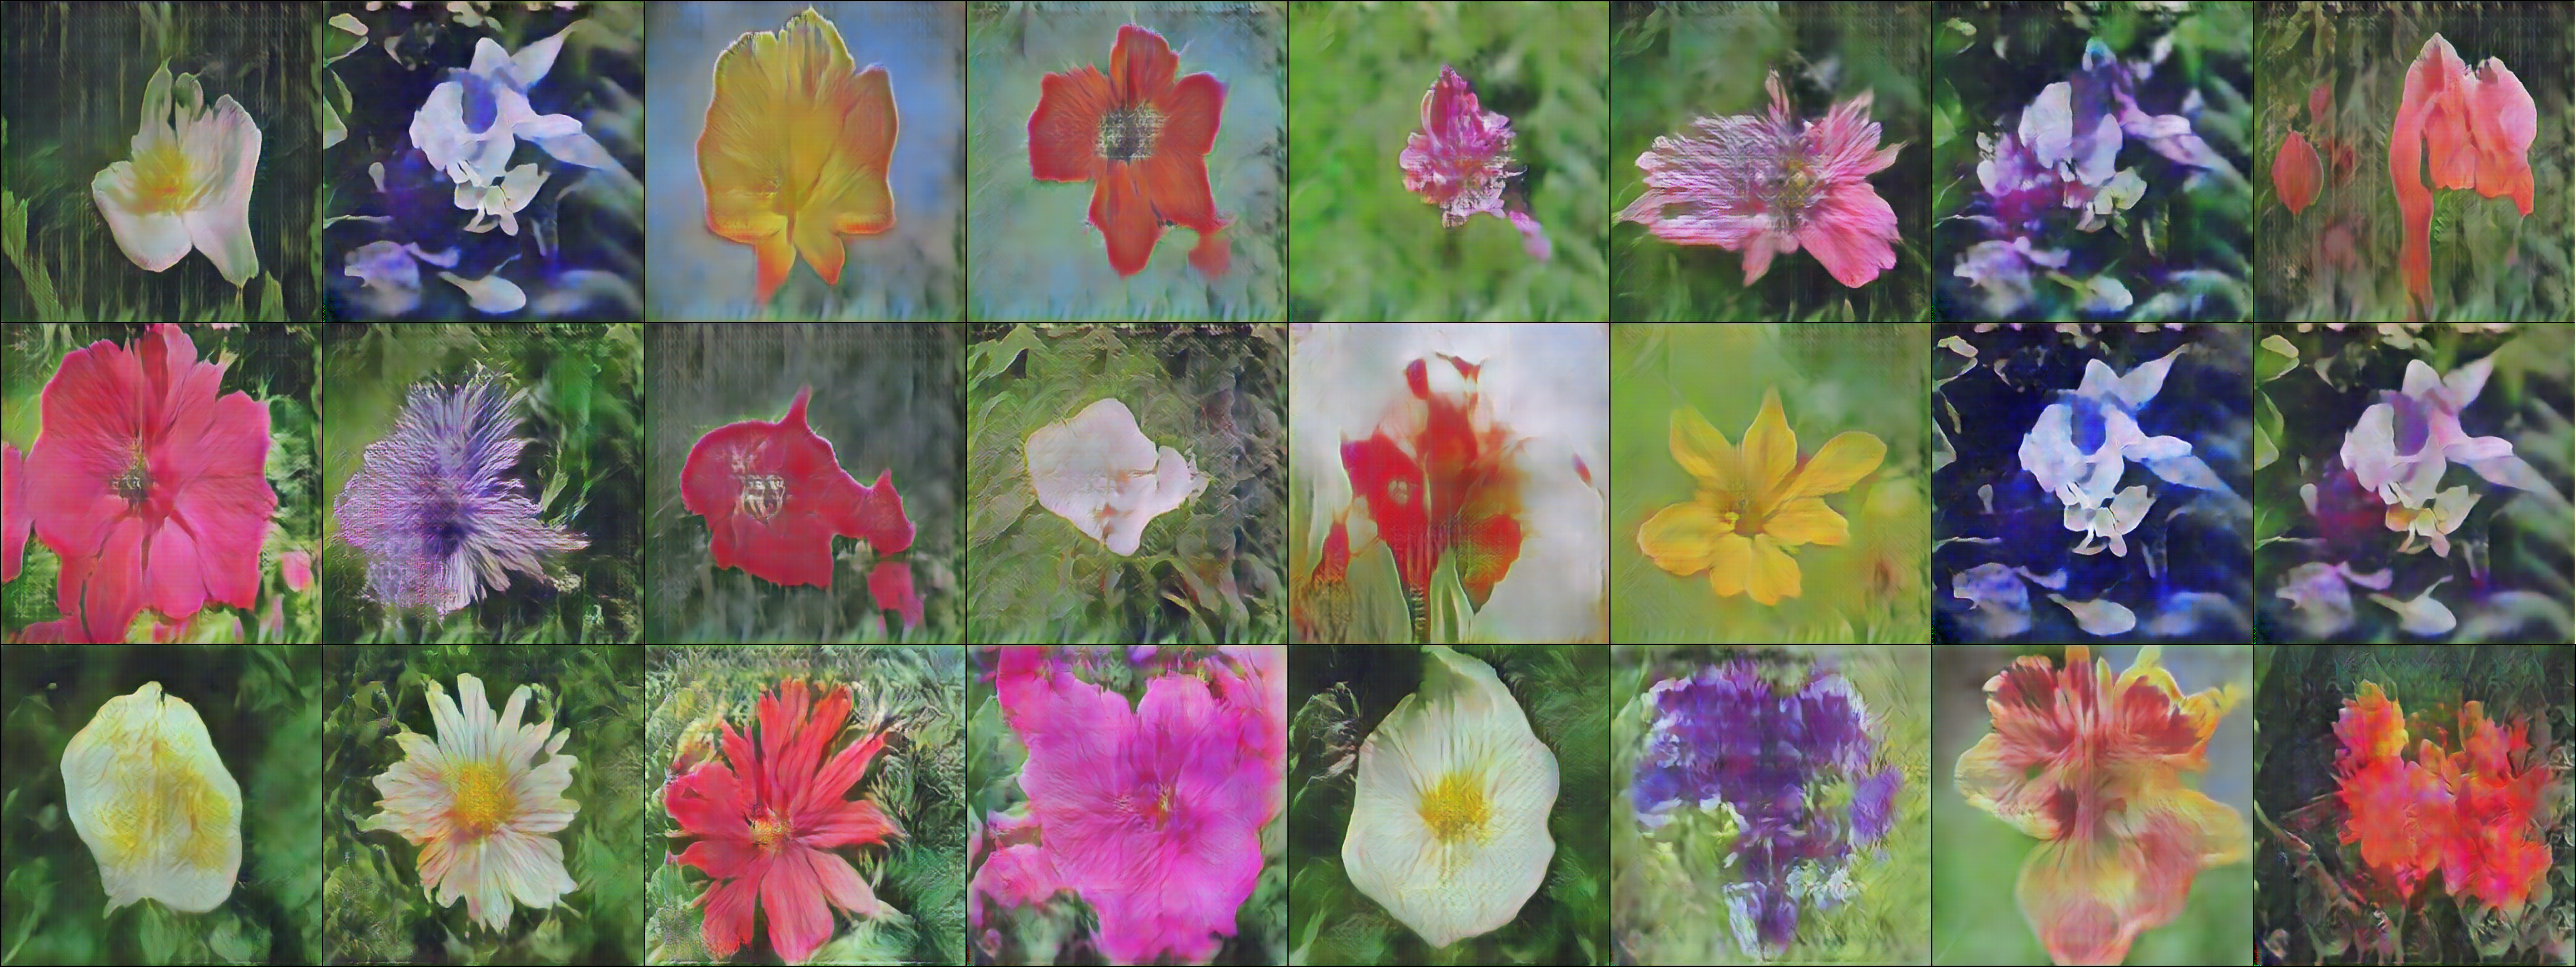
\includegraphics[width=.94\textwidth]{images/fake_samples_not_cherry_picked}
            \caption[not used]
            {
                \textbf{A collection of images that were generated with a DCGAN. The latent vectors used to produce these images were randomly sampled from the music dataset.}
            }
            \label{fig:dcgan_samples}
        \end{figure}

        blahblahblah

        \begin{figure}[ht]
            \centering
            \fbox{
                \includegraphics[width=.94\textwidth]{images/video_on_paper}
            }
            \caption[not used]
            {
                \textbf{\TODO{do}.}
            }
            \label{fig:video}
        \end{figure}
